\subsection{Regression}
\subsubsection{Without drift --- All-ones.}
\begin{figure}[H]
  \centering
  \begin{subfigure}[b]{0.48\textwidth}
    
\includegraphics[width=\textwidth]{figures/appendix/regression/nodrift/anyhow_all_ones/coverage_distribution}
    \caption{Coverage distribution}
  \end{subfigure}
  \hfill
  \begin{subfigure}[b]{0.48\textwidth}
    
\includegraphics[width=\textwidth]{figures/appendix/regression/nodrift/anyhow_all_ones/pvalue_trajectory}
    \caption{P-value trajectory}
  \end{subfigure}
  \medskip
  \begin{subfigure}[b]{0.48\textwidth}
    
\includegraphics[width=\textwidth]{figures/appendix/regression/nodrift/anyhow_all_ones/regression_bands}
    \caption{Regression bands}
  \end{subfigure}
  \hfill
  \begin{subfigure}[b]{0.48\textwidth}
    
\includegraphics[width=\textwidth]{figures/appendix/regression/nodrift/anyhow_all_ones/set_size_histogram}
    \caption{Set size histogram}
  \end{subfigure}
  \medskip
  \centering
  \begin{subfigure}[b]{0.48\textwidth}
    
\includegraphics[width=\textwidth]{figures/appendix/regression/nodrift/anyhow_all_ones/set_sizes_per_batch}
    \caption{Set sizes per batch}
  \end{subfigure}
  \caption{Regression, no drift, all-ones.}
  \label{fig:app-reg-nd-all-ones}
\end{figure}

\subsubsection{Without drift --- Window \texorpdfstring{$K{=}1$}{K=1}.}
\begin{figure}[H]
  \centering
  \begin{subfigure}[b]{0.48\textwidth}
    
\includegraphics[width=\textwidth]{figures/appendix/regression/nodrift/anyhow_window_1/coverage_distribution}
    \caption{Coverage distribution}
  \end{subfigure}
  \hfill
  \begin{subfigure}[b]{0.48\textwidth}
    
\includegraphics[width=\textwidth]{figures/appendix/regression/nodrift/anyhow_window_1/pvalue_trajectory}
    \caption{P-value trajectory}
  \end{subfigure}
  \medskip
  \begin{subfigure}[b]{0.48\textwidth}
    
\includegraphics[width=\textwidth]{figures/appendix/regression/nodrift/anyhow_window_1/regression_bands}
    \caption{Regression bands}
  \end{subfigure}
  \hfill
  \begin{subfigure}[b]{0.48\textwidth}
    
\includegraphics[width=\textwidth]{figures/appendix/regression/nodrift/anyhow_window_1/set_size_histogram}
    \caption{Set size histogram}
  \end{subfigure}
  \medskip
  \centering
  \begin{subfigure}[b]{0.48\textwidth}
    
\includegraphics[width=\textwidth]{figures/appendix/regression/nodrift/anyhow_window_1/set_sizes_per_batch}
    \caption{Set sizes per batch}
  \end{subfigure}
  \caption{Regression, no drift, window $K{=}1$.}
  \label{fig:app-reg-nd-window-1}
\end{figure}

\subsubsection{Without drift --- Window \texorpdfstring{$K{=}3$}{K=3}.}
\begin{figure}[H]
  \centering
  \begin{subfigure}[b]{0.48\textwidth}
    
\includegraphics[width=\textwidth]{figures/appendix/regression/nodrift/anyhow_window_3/coverage_distribution}
    \caption{Coverage distribution}
  \end{subfigure}
  \hfill
  \begin{subfigure}[b]{0.48\textwidth}
    
\includegraphics[width=\textwidth]{figures/appendix/regression/nodrift/anyhow_window_3/pvalue_trajectory}
    \caption{P-value trajectory}
  \end{subfigure}
  \medskip
  \begin{subfigure}[b]{0.48\textwidth}
    
\includegraphics[width=\textwidth]{figures/appendix/regression/nodrift/anyhow_window_3/regression_bands}
    \caption{Regression bands}
  \end{subfigure}
  \hfill
  \begin{subfigure}[b]{0.48\textwidth}
    
\includegraphics[width=\textwidth]{figures/appendix/regression/nodrift/anyhow_window_3/set_size_histogram}
    \caption{Set size histogram}
  \end{subfigure}
  \medskip
  \centering
  \begin{subfigure}[b]{0.48\textwidth}
    
\includegraphics[width=\textwidth]{figures/appendix/regression/nodrift/anyhow_window_3/set_sizes_per_batch}
    \caption{Set sizes per batch}
  \end{subfigure}
  \caption{Regression, no drift, window $K{=}3$.}
  \label{fig:app-reg-nd-window-3}
\end{figure}

\subsubsection{Without drift --- Window \texorpdfstring{$K{=}5$}{K=5}.}
\begin{figure}[H]
  \centering
  \begin{subfigure}[b]{0.48\textwidth}
    
\includegraphics[width=\textwidth]{figures/appendix/regression/nodrift/anyhow_window_5/coverage_distribution}
    \caption{Coverage distribution}
  \end{subfigure}
  \hfill
  \begin{subfigure}[b]{0.48\textwidth}
    
\includegraphics[width=\textwidth]{figures/appendix/regression/nodrift/anyhow_window_5/pvalue_trajectory}
    \caption{P-value trajectory}
  \end{subfigure}
  \medskip
  \begin{subfigure}[b]{0.48\textwidth}
    
\includegraphics[width=\textwidth]{figures/appendix/regression/nodrift/anyhow_window_5/regression_bands}
    \caption{Regression bands}
  \end{subfigure}
  \hfill
  \begin{subfigure}[b]{0.48\textwidth}
    
\includegraphics[width=\textwidth]{figures/appendix/regression/nodrift/anyhow_window_5/set_size_histogram}
    \caption{Set size histogram}
  \end{subfigure}
  \medskip
  \centering
  \begin{subfigure}[b]{0.48\textwidth}
    
\includegraphics[width=\textwidth]{figures/appendix/regression/nodrift/anyhow_window_5/set_sizes_per_batch}
    \caption{Set sizes per batch}
  \end{subfigure}
  \caption{Regression, no drift, window $K{=}5$.}
  \label{fig:app-reg-nd-window-5}
\end{figure}

\subsubsection{Without drift --- Window \texorpdfstring{$K{=}10$}{K=10}.}
\begin{figure}[H]
  \centering
  \begin{subfigure}[b]{0.48\textwidth}
    
\includegraphics[width=\textwidth]{figures/appendix/regression/nodrift/anyhow_window_10/coverage_distribution}
    \caption{Coverage distribution}
  \end{subfigure}
  \hfill
  \begin{subfigure}[b]{0.48\textwidth}
    
\includegraphics[width=\textwidth]{figures/appendix/regression/nodrift/anyhow_window_10/pvalue_trajectory}
    \caption{P-value trajectory}
  \end{subfigure}
  \medskip
  \begin{subfigure}[b]{0.48\textwidth}
    
\includegraphics[width=\textwidth]{figures/appendix/regression/nodrift/anyhow_window_10/regression_bands}
    \caption{Regression bands}
  \end{subfigure}
  \hfill
  \begin{subfigure}[b]{0.48\textwidth}
    
\includegraphics[width=\textwidth]{figures/appendix/regression/nodrift/anyhow_window_10/set_size_histogram}
    \caption{Set size histogram}
  \end{subfigure}
  \medskip
  \centering
  \begin{subfigure}[b]{0.48\textwidth}
    
\includegraphics[width=\textwidth]{figures/appendix/regression/nodrift/anyhow_window_10/set_sizes_per_batch}
    \caption{Set sizes per batch}
  \end{subfigure}
  \caption{Regression, no drift, window $K{=}10$.}
  \label{fig:app-reg-nd-window-10}
\end{figure}

\subsubsection{Without drift --- Window \texorpdfstring{$K{=}15$}{K=15}.}
\begin{figure}[H]
  \centering
  \begin{subfigure}[b]{0.48\textwidth}
    
\includegraphics[width=\textwidth]{figures/appendix/regression/nodrift/anyhow_window_15/coverage_distribution}
    \caption{Coverage distribution}
  \end{subfigure}
  \hfill
  \begin{subfigure}[b]{0.48\textwidth}
    
\includegraphics[width=\textwidth]{figures/appendix/regression/nodrift/anyhow_window_15/pvalue_trajectory}
    \caption{P-value trajectory}
  \end{subfigure}
  \medskip
  \begin{subfigure}[b]{0.48\textwidth}
    
\includegraphics[width=\textwidth]{figures/appendix/regression/nodrift/anyhow_window_15/regression_bands}
    \caption{Regression bands}
  \end{subfigure}
  \hfill
  \begin{subfigure}[b]{0.48\textwidth}
    
\includegraphics[width=\textwidth]{figures/appendix/regression/nodrift/anyhow_window_15/set_size_histogram}
    \caption{Set size histogram}
  \end{subfigure}
  \medskip
  \centering
  \begin{subfigure}[b]{0.48\textwidth}
    
\includegraphics[width=\textwidth]{figures/appendix/regression/nodrift/anyhow_window_15/set_sizes_per_batch}
    \caption{Set sizes per batch}
  \end{subfigure}
  \caption{Regression, no drift, window $K{=}15$.}
  \label{fig:app-reg-nd-window-15}
\end{figure}

\subsubsection{Without drift --- Window \texorpdfstring{$K{=}25$}{K=25}.}
\begin{figure}[H]
  \centering
  \begin{subfigure}[b]{0.48\textwidth}
    
\includegraphics[width=\textwidth]{figures/appendix/regression/nodrift/anyhow_window_25/coverage_distribution}
    \caption{Coverage distribution}
  \end{subfigure}
  \hfill
  \begin{subfigure}[b]{0.48\textwidth}
    
\includegraphics[width=\textwidth]{figures/appendix/regression/nodrift/anyhow_window_25/pvalue_trajectory}
    \caption{P-value trajectory}
  \end{subfigure}
  \medskip
  \begin{subfigure}[b]{0.48\textwidth}
    
\includegraphics[width=\textwidth]{figures/appendix/regression/nodrift/anyhow_window_25/regression_bands}
    \caption{Regression bands}
  \end{subfigure}
  \hfill
  \begin{subfigure}[b]{0.48\textwidth}
    
\includegraphics[width=\textwidth]{figures/appendix/regression/nodrift/anyhow_window_25/set_size_histogram}
    \caption{Set size histogram}
  \end{subfigure}
  \medskip
  \centering
  \begin{subfigure}[b]{0.48\textwidth}
    
\includegraphics[width=\textwidth]{figures/appendix/regression/nodrift/anyhow_window_25/set_sizes_per_batch}
    \caption{Set sizes per batch}
  \end{subfigure}
  \caption{Regression, no drift, window $K{=}25$.}
  \label{fig:app-reg-nd-window-25}
\end{figure}

\subsubsection{With drift --- All-ones.}
\begin{figure}[H]
  \centering
  \begin{subfigure}[b]{0.48\textwidth}
    
\includegraphics[width=\textwidth]{figures/appendix/regression/drift/anyhow_all_ones/coverage_distribution}
    \caption{Coverage distribution}
  \end{subfigure}
  \hfill
  \begin{subfigure}[b]{0.48\textwidth}
    
\includegraphics[width=\textwidth]{figures/appendix/regression/drift/anyhow_all_ones/pvalue_trajectory}
    \caption{P-value trajectory}
  \end{subfigure}
  \medskip
  \begin{subfigure}[b]{0.48\textwidth}
    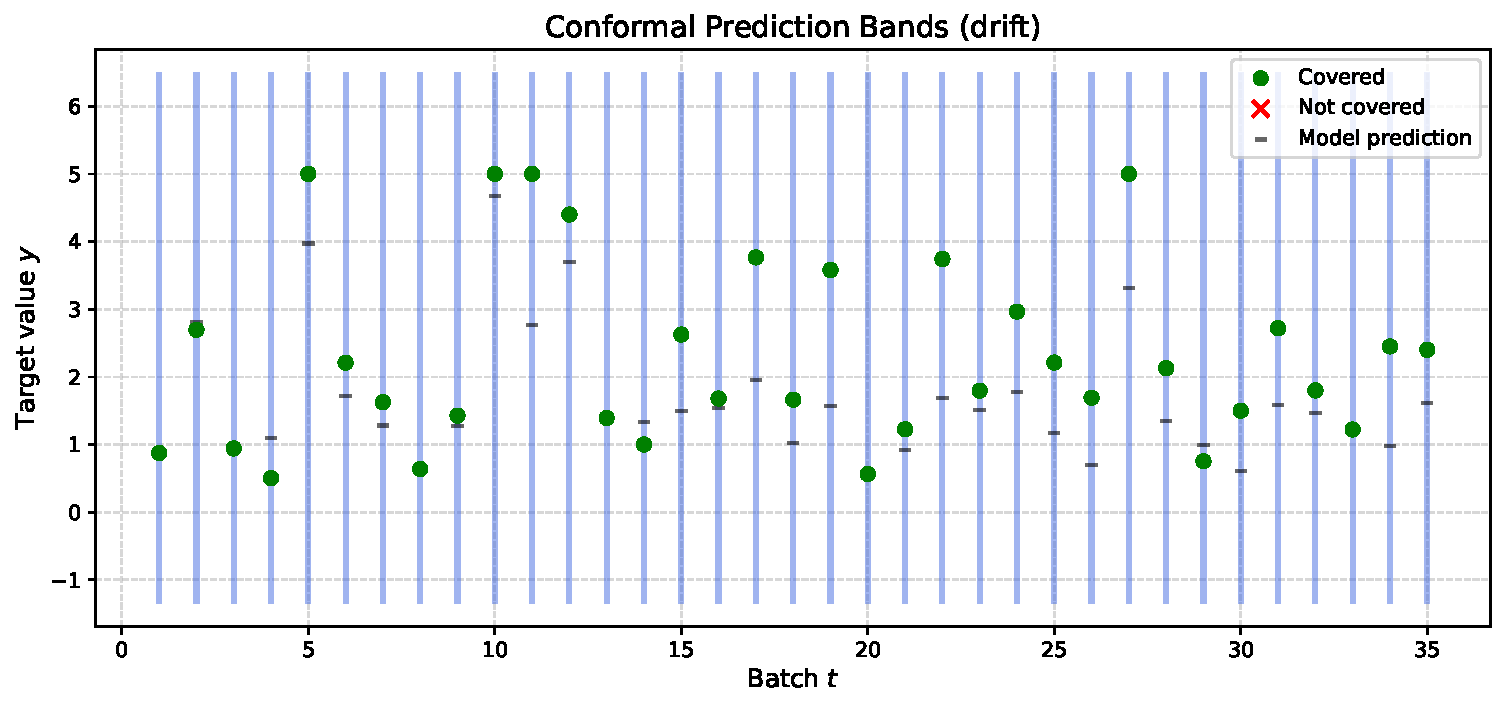
\includegraphics[width=\textwidth]{figures/appendix/regression/drift/anyhow_all_ones/regression_bands}
    \caption{Regression bands}
  \end{subfigure}
  \hfill
  \begin{subfigure}[b]{0.48\textwidth}
    
\includegraphics[width=\textwidth]{figures/appendix/regression/drift/anyhow_all_ones/set_size_histogram}
    \caption{Set size histogram}
  \end{subfigure}
  \medskip
  \centering
  \begin{subfigure}[b]{0.48\textwidth}
    
\includegraphics[width=\textwidth]{figures/appendix/regression/drift/anyhow_all_ones/set_sizes_per_batch}
    \caption{Set sizes per batch}
  \end{subfigure}
  \caption{Regression, drift, all-ones.}
  \label{fig:app-reg-d-all-ones}
\end{figure}

\subsubsection{With drift --- Window \texorpdfstring{$K{=}1$}{K=1}.}
\begin{figure}[H]
  \centering
  \begin{subfigure}[b]{0.48\textwidth}
    
\includegraphics[width=\textwidth]{figures/appendix/regression/drift/anyhow_window_1/coverage_distribution}
    \caption{Coverage distribution}
  \end{subfigure}
  \hfill
  \begin{subfigure}[b]{0.48\textwidth}
    
\includegraphics[width=\textwidth]{figures/appendix/regression/drift/anyhow_window_1/pvalue_trajectory}
    \caption{P-value trajectory}
  \end{subfigure}
  \medskip
  \begin{subfigure}[b]{0.48\textwidth}
    
\includegraphics[width=\textwidth]{figures/appendix/regression/drift/anyhow_window_1/regression_bands}
    \caption{Regression bands}
  \end{subfigure}
  \hfill
  \begin{subfigure}[b]{0.48\textwidth}
    
\includegraphics[width=\textwidth]{figures/appendix/regression/drift/anyhow_window_1/set_size_histogram}
    \caption{Set size histogram}
  \end{subfigure}
  \medskip
  \centering
  \begin{subfigure}[b]{0.48\textwidth}
    
\includegraphics[width=\textwidth]{figures/appendix/regression/drift/anyhow_window_1/set_sizes_per_batch}
    \caption{Set sizes per batch}
  \end{subfigure}
  \caption{Regression, drift, window $K{=}1$.}
  \label{fig:app-reg-d-window-1}
\end{figure}

\subsubsection{With drift --- Window \texorpdfstring{$K{=}3$}{K=3}.}
\begin{figure}[H]
  \centering
  \begin{subfigure}[b]{0.48\textwidth}
    
\includegraphics[width=\textwidth]{figures/appendix/regression/drift/anyhow_window_3/coverage_distribution}
    \caption{Coverage distribution}
  \end{subfigure}
  \hfill
  \begin{subfigure}[b]{0.48\textwidth}
    
\includegraphics[width=\textwidth]{figures/appendix/regression/drift/anyhow_window_3/pvalue_trajectory}
    \caption{P-value trajectory}
  \end{subfigure}
  \medskip
  \begin{subfigure}[b]{0.48\textwidth}
    
\includegraphics[width=\textwidth]{figures/appendix/regression/drift/anyhow_window_3/regression_bands}
    \caption{Regression bands}
  \end{subfigure}
  \hfill
  \begin{subfigure}[b]{0.48\textwidth}
    
\includegraphics[width=\textwidth]{figures/appendix/regression/drift/anyhow_window_3/set_size_histogram}
    \caption{Set size histogram}
  \end{subfigure}
  \medskip
  \centering
  \begin{subfigure}[b]{0.48\textwidth}
    
\includegraphics[width=\textwidth]{figures/appendix/regression/drift/anyhow_window_3/set_sizes_per_batch}
    \caption{Set sizes per batch}
  \end{subfigure}
  \caption{Regression, drift, window $K{=}3$.}
  \label{fig:app-reg-d-window-3}
\end{figure}

\subsubsection{With drift --- Window \texorpdfstring{$K{=}5$}{K=5}.}
\begin{figure}[H]
  \centering
  \begin{subfigure}[b]{0.48\textwidth}
    
\includegraphics[width=\textwidth]{figures/appendix/regression/drift/anyhow_window_5/coverage_distribution}
    \caption{Coverage distribution}
  \end{subfigure}
  \hfill
  \begin{subfigure}[b]{0.48\textwidth}
    
\includegraphics[width=\textwidth]{figures/appendix/regression/drift/anyhow_window_5/pvalue_trajectory}
    \caption{P-value trajectory}
  \end{subfigure}
  \medskip
  \begin{subfigure}[b]{0.48\textwidth}
    
\includegraphics[width=\textwidth]{figures/appendix/regression/drift/anyhow_window_5/regression_bands}
    \caption{Regression bands}
  \end{subfigure}
  \hfill
  \begin{subfigure}[b]{0.48\textwidth}
    
\includegraphics[width=\textwidth]{figures/appendix/regression/drift/anyhow_window_5/set_size_histogram}
    \caption{Set size histogram}
  \end{subfigure}
  \medskip
  \centering
  \begin{subfigure}[b]{0.48\textwidth}
    
\includegraphics[width=\textwidth]{figures/appendix/regression/drift/anyhow_window_5/set_sizes_per_batch}
    \caption{Set sizes per batch}
  \end{subfigure}
  \caption{Regression, drift, window $K{=}5$.}
  \label{fig:app-reg-d-window-5}
\end{figure}

\subsubsection{With drift --- Window \texorpdfstring{$K{=}10$}{K=10}.}
\begin{figure}[H]
  \centering
  \begin{subfigure}[b]{0.48\textwidth}
    
\includegraphics[width=\textwidth]{figures/appendix/regression/drift/anyhow_window_10/coverage_distribution}
    \caption{Coverage distribution}
  \end{subfigure}
  \hfill
  \begin{subfigure}[b]{0.48\textwidth}
    
\includegraphics[width=\textwidth]{figures/appendix/regression/drift/anyhow_window_10/pvalue_trajectory}
    \caption{P-value trajectory}
  \end{subfigure}
  \medskip
  \begin{subfigure}[b]{0.48\textwidth}
    
\includegraphics[width=\textwidth]{figures/appendix/regression/drift/anyhow_window_10/regression_bands}
    \caption{Regression bands}
  \end{subfigure}
  \hfill
  \begin{subfigure}[b]{0.48\textwidth}
    
\includegraphics[width=\textwidth]{figures/appendix/regression/drift/anyhow_window_10/set_size_histogram}
    \caption{Set size histogram}
  \end{subfigure}
  \medskip
  \centering
  \begin{subfigure}[b]{0.48\textwidth}
    
\includegraphics[width=\textwidth]{figures/appendix/regression/drift/anyhow_window_10/set_sizes_per_batch}
    \caption{Set sizes per batch}
  \end{subfigure}
  \caption{Regression, drift, window $K{=}10$.}
  \label{fig:app-reg-d-window-10}
\end{figure}

\subsubsection{With drift --- Window \texorpdfstring{$K{=}15$}{K=15}.}
\begin{figure}[H]
  \centering
  \begin{subfigure}[b]{0.48\textwidth}
    
\includegraphics[width=\textwidth]{figures/appendix/regression/drift/anyhow_window_15/coverage_distribution}
    \caption{Coverage distribution}
  \end{subfigure}
  \hfill
  \begin{subfigure}[b]{0.48\textwidth}
    
\includegraphics[width=\textwidth]{figures/appendix/regression/drift/anyhow_window_15/pvalue_trajectory}
    \caption{P-value trajectory}
  \end{subfigure}
  \medskip
  \begin{subfigure}[b]{0.48\textwidth}
    
\includegraphics[width=\textwidth]{figures/appendix/regression/drift/anyhow_window_15/regression_bands}
    \caption{Regression bands}
  \end{subfigure}
  \hfill
  \begin{subfigure}[b]{0.48\textwidth}
    
\includegraphics[width=\textwidth]{figures/appendix/regression/drift/anyhow_window_15/set_size_histogram}
    \caption{Set size histogram}
  \end{subfigure}
  \medskip
  \centering
  \begin{subfigure}[b]{0.48\textwidth}
    
\includegraphics[width=\textwidth]{figures/appendix/regression/drift/anyhow_window_15/set_sizes_per_batch}
    \caption{Set sizes per batch}
  \end{subfigure}
  \caption{Regression, drift, window $K{=}15$.}
  \label{fig:app-reg-d-window-15}
\end{figure}

\subsubsection{With drift --- Window \texorpdfstring{$K{=}25$}{K=25}.}
\begin{figure}[H]
  \centering
  \begin{subfigure}[b]{0.48\textwidth}
    
\includegraphics[width=\textwidth]{figures/appendix/regression/drift/anyhow_window_25/coverage_distribution}
    \caption{Coverage distribution}
  \end{subfigure}
  \hfill
  \begin{subfigure}[b]{0.48\textwidth}
    
\includegraphics[width=\textwidth]{figures/appendix/regression/drift/anyhow_window_25/pvalue_trajectory}
    \caption{P-value trajectory}
  \end{subfigure}
  \medskip
  \begin{subfigure}[b]{0.48\textwidth}
    
\includegraphics[width=\textwidth]{figures/appendix/regression/drift/anyhow_window_25/regression_bands}
    \caption{Regression bands}
  \end{subfigure}
  \hfill
  \begin{subfigure}[b]{0.48\textwidth}
    
\includegraphics[width=\textwidth]{figures/appendix/regression/drift/anyhow_window_25/set_size_histogram}
    \caption{Set size histogram}
  \end{subfigure}
  \medskip
  \centering
  \begin{subfigure}[b]{0.48\textwidth}
    
\includegraphics[width=\textwidth]{figures/appendix/regression/drift/anyhow_window_25/set_sizes_per_batch}
    \caption{Set sizes per batch}
  \end{subfigure}
  \caption{Regression, drift, window $K{=}25$.}
  \label{fig:app-reg-d-window-25}
\end{figure}

\subsection{Classification}
\subsubsection{Without drift --- All-ones.}
\begin{figure}[H]
  \centering
  \begin{subfigure}[b]{0.48\textwidth}
    
\includegraphics[width=\textwidth]{figures/appendix/classification/nodrift/anyhow_all_ones/coverage_distribution}
    \caption{Coverage distribution}
  \end{subfigure}
  \hfill
  \begin{subfigure}[b]{0.48\textwidth}
    
\includegraphics[width=\textwidth]{figures/appendix/classification/nodrift/anyhow_all_ones/pvalue_trajectory}
    \caption{P-value trajectory}
  \end{subfigure}
  \medskip
  \begin{subfigure}[b]{0.48\textwidth}
    
\includegraphics[width=\textwidth]{figures/appendix/classification/nodrift/anyhow_all_ones/conformal_sequence_matrix}
    \caption{Conformal sequence matrix}
  \end{subfigure}
  \hfill
  \begin{subfigure}[b]{0.48\textwidth}
    
\includegraphics[width=\textwidth]{figures/appendix/classification/nodrift/anyhow_all_ones/set_size_histogram}
    \caption{Set size histogram}
  \end{subfigure}
  \medskip
  \centering
  \begin{subfigure}[b]{0.48\textwidth}
    
\includegraphics[width=\textwidth]{figures/appendix/classification/nodrift/anyhow_all_ones/set_sizes_per_batch}
    \caption{Set sizes per batch}
  \end{subfigure}
  \caption{Classification, no drift, all-ones.}
  \label{fig:app-cla-nd-all-ones}
\end{figure}

\subsubsection{Without drift --- Window \texorpdfstring{$K{=}1$}{K=1}.}
\begin{figure}[H]
  \centering
  \begin{subfigure}[b]{0.48\textwidth}
    
\includegraphics[width=\textwidth]{figures/appendix/classification/nodrift/anyhow_window_1/coverage_distribution}
    \caption{Coverage distribution}
  \end{subfigure}
  \hfill
  \begin{subfigure}[b]{0.48\textwidth}
    
\includegraphics[width=\textwidth]{figures/appendix/classification/nodrift/anyhow_window_1/pvalue_trajectory}
    \caption{P-value trajectory}
  \end{subfigure}
  \medskip
  \begin{subfigure}[b]{0.48\textwidth}
    
\includegraphics[width=\textwidth]{figures/appendix/classification/nodrift/anyhow_window_1/conformal_sequence_matrix}
    \caption{Conformal sequence matrix}
  \end{subfigure}
  \hfill
  \begin{subfigure}[b]{0.48\textwidth}
    
\includegraphics[width=\textwidth]{figures/appendix/classification/nodrift/anyhow_window_1/set_size_histogram}
    \caption{Set size histogram}
  \end{subfigure}
  \medskip
  \centering
  \begin{subfigure}[b]{0.48\textwidth}
    
\includegraphics[width=\textwidth]{figures/appendix/classification/nodrift/anyhow_window_1/set_sizes_per_batch}
    \caption{Set sizes per batch}
  \end{subfigure}
  \caption{Classification, no drift, window $K{=}1$.}
  \label{fig:app-cla-nd-window-1}
\end{figure}

\subsubsection{Without drift --- Window \texorpdfstring{$K{=}3$}{K=3}.}
\begin{figure}[H]
  \centering
  \begin{subfigure}[b]{0.48\textwidth}
    
\includegraphics[width=\textwidth]{figures/appendix/classification/nodrift/anyhow_window_3/coverage_distribution}
    \caption{Coverage distribution}
  \end{subfigure}
  \hfill
  \begin{subfigure}[b]{0.48\textwidth}
    
\includegraphics[width=\textwidth]{figures/appendix/classification/nodrift/anyhow_window_3/pvalue_trajectory}
    \caption{P-value trajectory}
  \end{subfigure}
  \medskip
  \begin{subfigure}[b]{0.48\textwidth}
    
\includegraphics[width=\textwidth]{figures/appendix/classification/nodrift/anyhow_window_3/conformal_sequence_matrix}
    \caption{Conformal sequence matrix}
  \end{subfigure}
  \hfill
  \begin{subfigure}[b]{0.48\textwidth}
    
\includegraphics[width=\textwidth]{figures/appendix/classification/nodrift/anyhow_window_3/set_size_histogram}
    \caption{Set size histogram}
  \end{subfigure}
  \medskip
  \centering
  \begin{subfigure}[b]{0.48\textwidth}
    
\includegraphics[width=\textwidth]{figures/appendix/classification/nodrift/anyhow_window_3/set_sizes_per_batch}
    \caption{Set sizes per batch}
  \end{subfigure}
  \caption{Classification, no drift, window $K{=}3$.}
  \label{fig:app-cla-nd-window-3}
\end{figure}

\subsubsection{Without drift --- Window \texorpdfstring{$K{=}5$}{K=5}.}
\begin{figure}[H]
  \centering
  \begin{subfigure}[b]{0.48\textwidth}
    
\includegraphics[width=\textwidth]{figures/appendix/classification/nodrift/anyhow_window_5/coverage_distribution}
    \caption{Coverage distribution}
  \end{subfigure}
  \hfill
  \begin{subfigure}[b]{0.48\textwidth}
    
\includegraphics[width=\textwidth]{figures/appendix/classification/nodrift/anyhow_window_5/pvalue_trajectory}
    \caption{P-value trajectory}
  \end{subfigure}
  \medskip
  \begin{subfigure}[b]{0.48\textwidth}
    
\includegraphics[width=\textwidth]{figures/appendix/classification/nodrift/anyhow_window_5/conformal_sequence_matrix}
    \caption{Conformal sequence matrix}
  \end{subfigure}
  \hfill
  \begin{subfigure}[b]{0.48\textwidth}
    
\includegraphics[width=\textwidth]{figures/appendix/classification/nodrift/anyhow_window_5/set_size_histogram}
    \caption{Set size histogram}
  \end{subfigure}
  \medskip
  \centering
  \begin{subfigure}[b]{0.48\textwidth}
    
\includegraphics[width=\textwidth]{figures/appendix/classification/nodrift/anyhow_window_5/set_sizes_per_batch}
    \caption{Set sizes per batch}
  \end{subfigure}
  \caption{Classification, no drift, window $K{=}5$.}
  \label{fig:app-cla-nd-window-5}
\end{figure}

\subsubsection{Without drift --- Window \texorpdfstring{$K{=}10$}{K=10}.}
\begin{figure}[H]
  \centering
  \begin{subfigure}[b]{0.48\textwidth}
    
\includegraphics[width=\textwidth]{figures/appendix/classification/nodrift/anyhow_window_10/coverage_distribution}
    \caption{Coverage distribution}
  \end{subfigure}
  \hfill
  \begin{subfigure}[b]{0.48\textwidth}
    
\includegraphics[width=\textwidth]{figures/appendix/classification/nodrift/anyhow_window_10/pvalue_trajectory}
    \caption{P-value trajectory}
  \end{subfigure}
  \medskip
  \begin{subfigure}[b]{0.48\textwidth}
    
\includegraphics[width=\textwidth]{figures/appendix/classification/nodrift/anyhow_window_10/conformal_sequence_matrix}
    \caption{Conformal sequence matrix}
  \end{subfigure}
  \hfill
  \begin{subfigure}[b]{0.48\textwidth}
    
\includegraphics[width=\textwidth]{figures/appendix/classification/nodrift/anyhow_window_10/set_size_histogram}
    \caption{Set size histogram}
  \end{subfigure}
  \medskip
  \centering
  \begin{subfigure}[b]{0.48\textwidth}
    
\includegraphics[width=\textwidth]{figures/appendix/classification/nodrift/anyhow_window_10/set_sizes_per_batch}
    \caption{Set sizes per batch}
  \end{subfigure}
  \caption{Classification, no drift, window $K{=}10$.}
  \label{fig:app-cla-nd-window-10}
\end{figure}

\subsubsection{Without drift --- Window \texorpdfstring{$K{=}15$}{K=15}.}
\begin{figure}[H]
  \centering
  \begin{subfigure}[b]{0.48\textwidth}
    
\includegraphics[width=\textwidth]{figures/appendix/classification/nodrift/anyhow_window_15/coverage_distribution}
    \caption{Coverage distribution}
  \end{subfigure}
  \hfill
  \begin{subfigure}[b]{0.48\textwidth}
    
\includegraphics[width=\textwidth]{figures/appendix/classification/nodrift/anyhow_window_15/pvalue_trajectory}
    \caption{P-value trajectory}
  \end{subfigure}
  \medskip
  \begin{subfigure}[b]{0.48\textwidth}
    
\includegraphics[width=\textwidth]{figures/appendix/classification/nodrift/anyhow_window_15/conformal_sequence_matrix}
    \caption{Conformal sequence matrix}
  \end{subfigure}
  \hfill
  \begin{subfigure}[b]{0.48\textwidth}
    
\includegraphics[width=\textwidth]{figures/appendix/classification/nodrift/anyhow_window_15/set_size_histogram}
    \caption{Set size histogram}
  \end{subfigure}
  \medskip
  \centering
  \begin{subfigure}[b]{0.48\textwidth}
    
\includegraphics[width=\textwidth]{figures/appendix/classification/nodrift/anyhow_window_15/set_sizes_per_batch}
    \caption{Set sizes per batch}
  \end{subfigure}
  \caption{Classification, no drift, window $K{=}15$.}
  \label{fig:app-cla-nd-window-15}
\end{figure}

\subsubsection{Without drift --- Window \texorpdfstring{$K{=}25$}{K=25}.}
\begin{figure}[H]
  \centering
  \begin{subfigure}[b]{0.48\textwidth}
    
\includegraphics[width=\textwidth]{figures/appendix/classification/nodrift/anyhow_window_25/coverage_distribution}
    \caption{Coverage distribution}
  \end{subfigure}
  \hfill
  \begin{subfigure}[b]{0.48\textwidth}
    
\includegraphics[width=\textwidth]{figures/appendix/classification/nodrift/anyhow_window_25/pvalue_trajectory}
    \caption{P-value trajectory}
  \end{subfigure}
  \medskip
  \begin{subfigure}[b]{0.48\textwidth}
    
\includegraphics[width=\textwidth]{figures/appendix/classification/nodrift/anyhow_window_25/conformal_sequence_matrix}
    \caption{Conformal sequence matrix}
  \end{subfigure}
  \hfill
  \begin{subfigure}[b]{0.48\textwidth}
    
\includegraphics[width=\textwidth]{figures/appendix/classification/nodrift/anyhow_window_25/set_size_histogram}
    \caption{Set size histogram}
  \end{subfigure}
  \medskip
  \centering
  \begin{subfigure}[b]{0.48\textwidth}
    
\includegraphics[width=\textwidth]{figures/appendix/classification/nodrift/anyhow_window_25/set_sizes_per_batch}
    \caption{Set sizes per batch}
  \end{subfigure}
  \caption{Classification, no drift, window $K{=}25$.}
  \label{fig:app-cla-nd-window-25}
\end{figure}

\subsubsection{With drift --- All-ones.}
\begin{figure}[H]
  \centering
  \begin{subfigure}[b]{0.48\textwidth}
    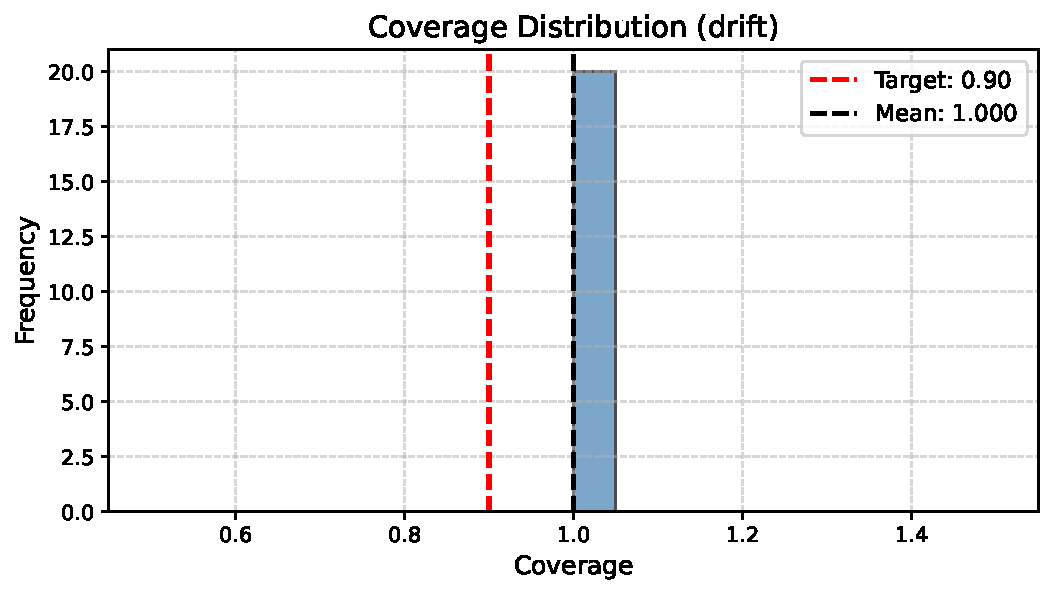
\includegraphics[width=\textwidth]{figures/appendix/classification/drift/anyhow_all_ones/coverage_distribution}
    \caption{Coverage distribution}
  \end{subfigure}
  \hfill
  \begin{subfigure}[b]{0.48\textwidth}
    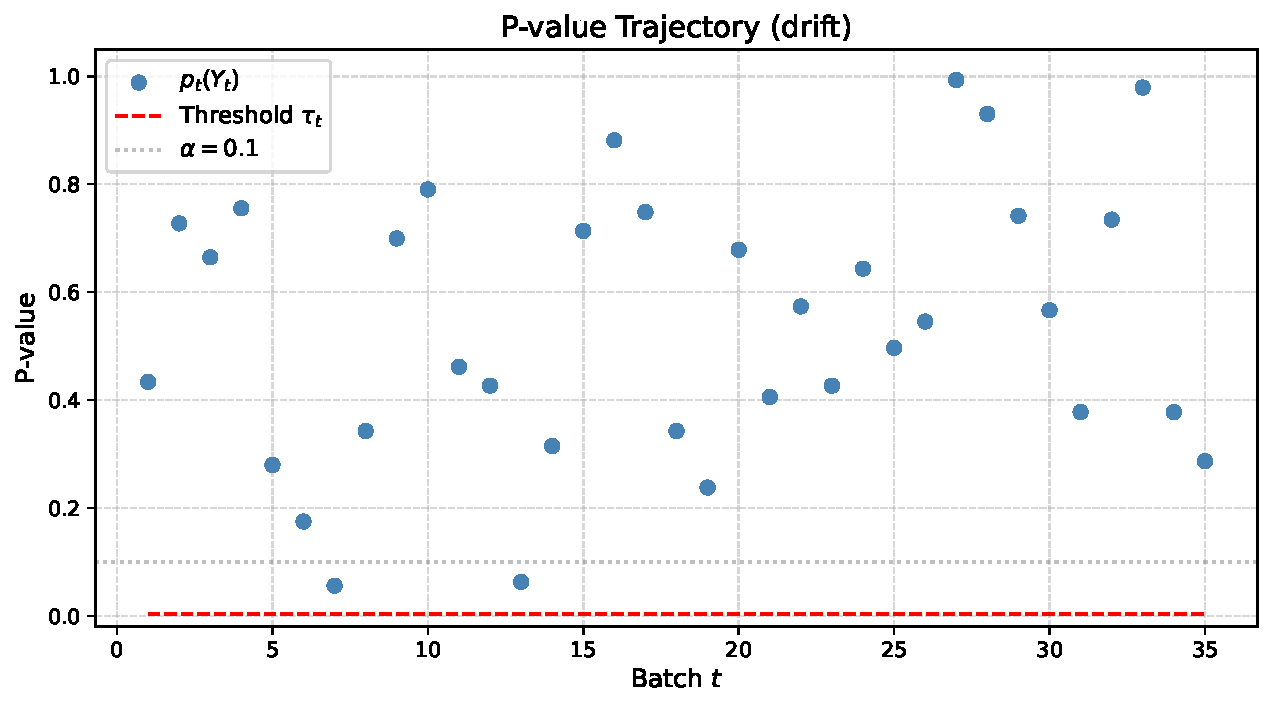
\includegraphics[width=\textwidth]{figures/appendix/classification/drift/anyhow_all_ones/pvalue_trajectory}
    \caption{P-value trajectory}
  \end{subfigure}
  \medskip
  \begin{subfigure}[b]{0.48\textwidth}
    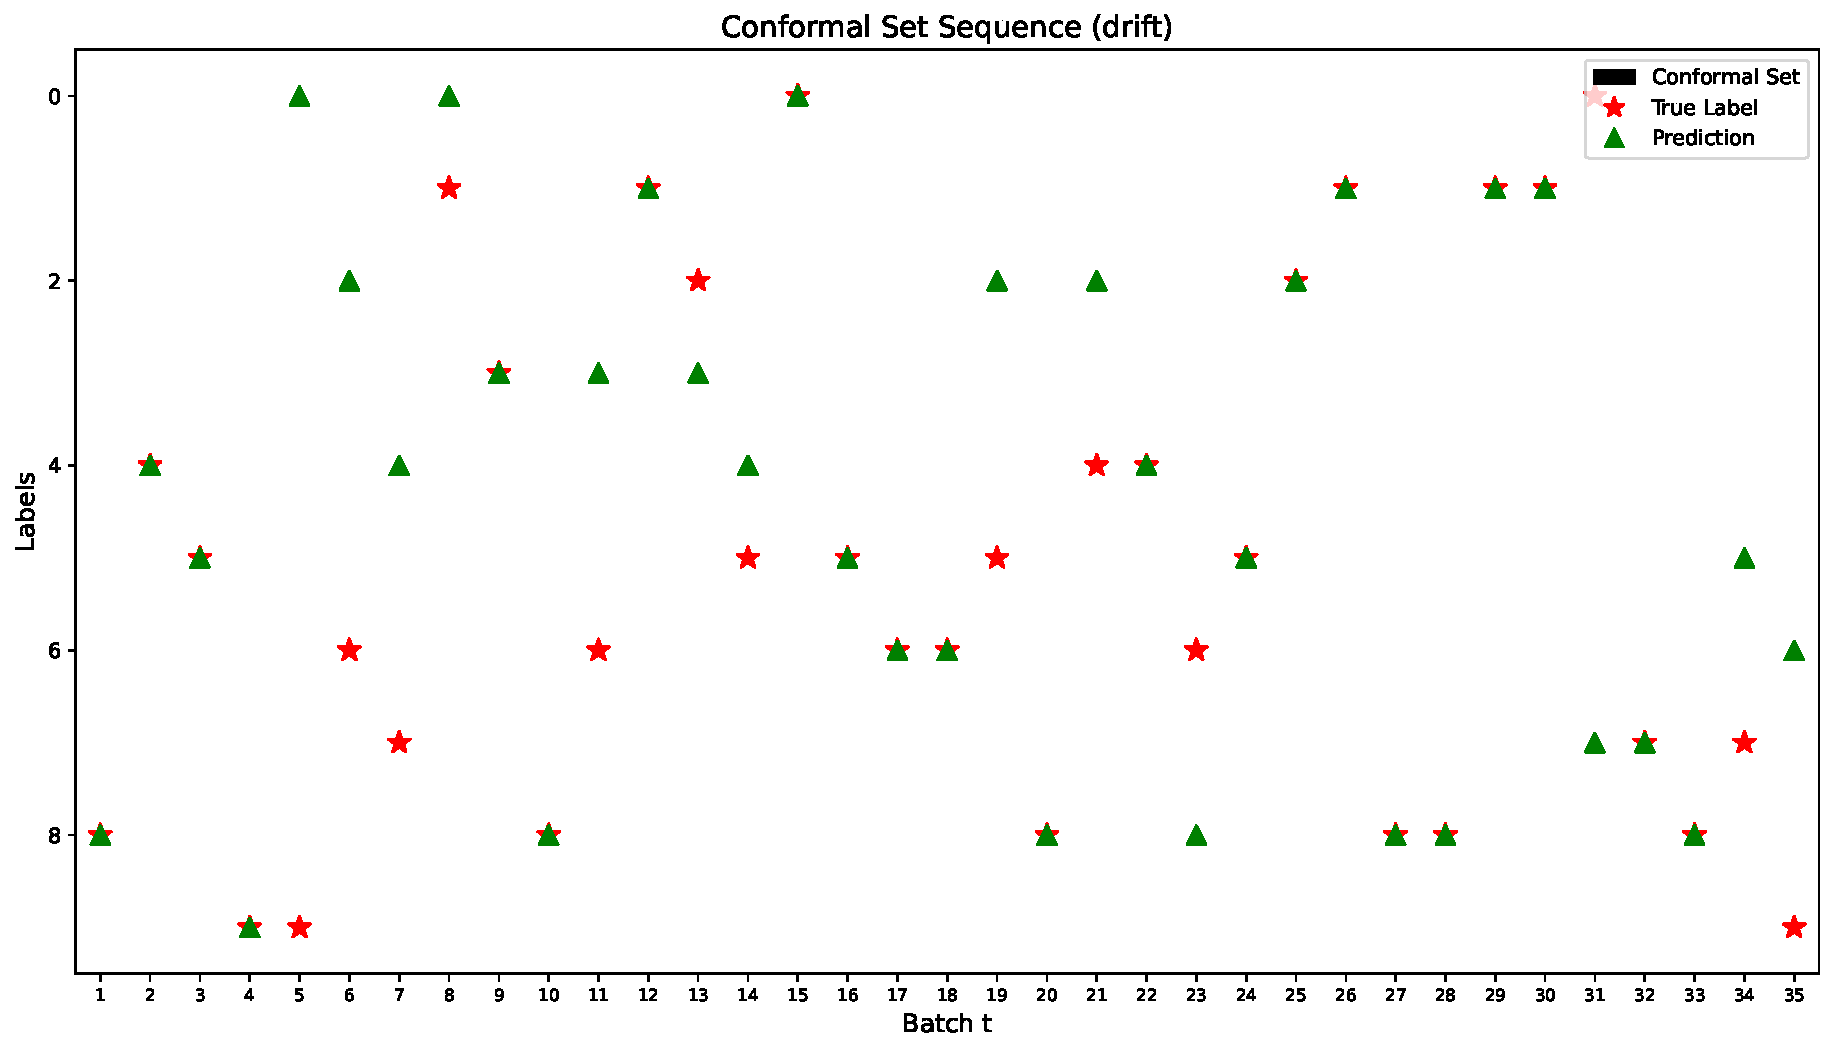
\includegraphics[width=\textwidth]{figures/appendix/classification/drift/anyhow_all_ones/conformal_sequence_matrix}
    \caption{Conformal sequence matrix}
  \end{subfigure}
  \hfill
  \begin{subfigure}[b]{0.48\textwidth}
    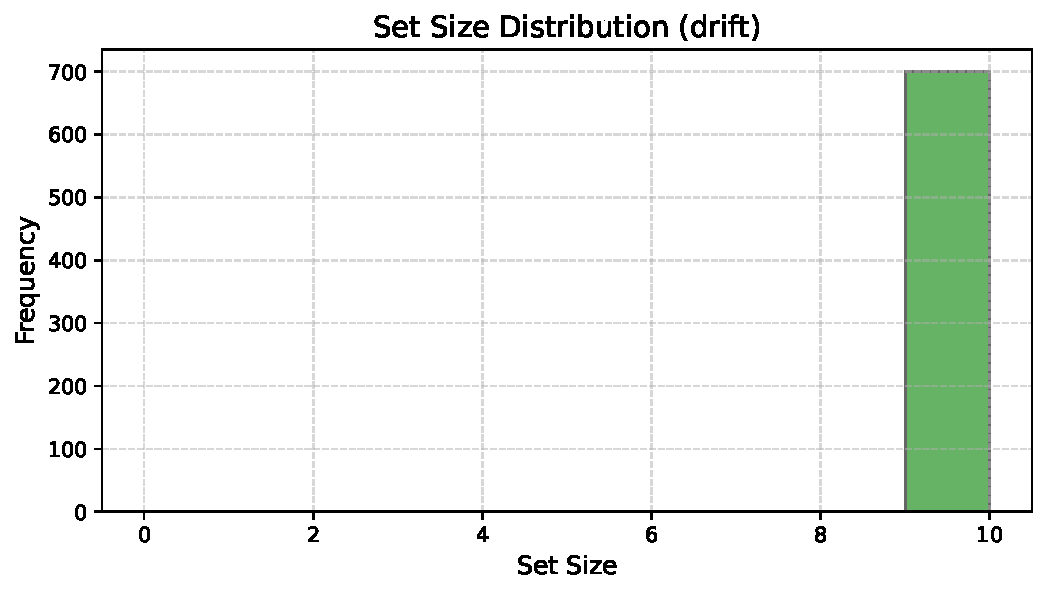
\includegraphics[width=\textwidth]{figures/appendix/classification/drift/anyhow_all_ones/set_size_histogram}
    \caption{Set size histogram}
  \end{subfigure}
  \medskip
  \centering
  \begin{subfigure}[b]{0.48\textwidth}
    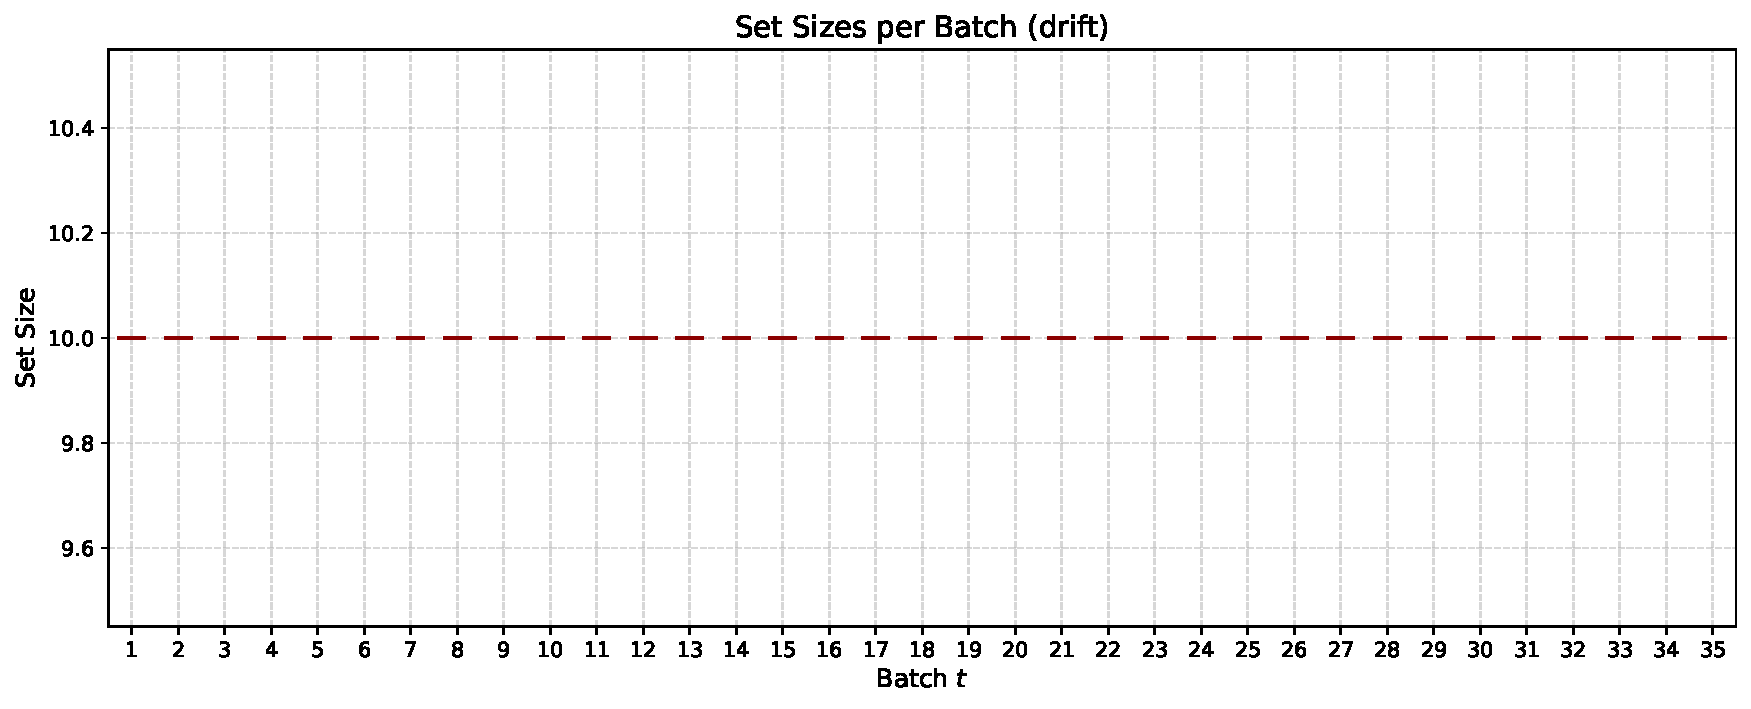
\includegraphics[width=\textwidth]{figures/appendix/classification/drift/anyhow_all_ones/set_sizes_per_batch}
    \caption{Set sizes per batch}
  \end{subfigure}
  \caption{Classification, drift, all-ones.}
  \label{fig:app-cla-d-all-ones}
\end{figure}

\subsubsection{With drift --- Window \texorpdfstring{$K{=}1$}{K=1}.}
\begin{figure}[H]
  \centering
  \begin{subfigure}[b]{0.48\textwidth}
    
\includegraphics[width=\textwidth]{figures/appendix/classification/drift/anyhow_window_1/coverage_distribution}
    \caption{Coverage distribution}
  \end{subfigure}
  \hfill
  \begin{subfigure}[b]{0.48\textwidth}
    
\includegraphics[width=\textwidth]{figures/appendix/classification/drift/anyhow_window_1/pvalue_trajectory}
    \caption{P-value trajectory}
  \end{subfigure}
  \medskip
  \begin{subfigure}[b]{0.48\textwidth}
    
\includegraphics[width=\textwidth]{figures/appendix/classification/drift/anyhow_window_1/conformal_sequence_matrix}
    \caption{Conformal sequence matrix}
  \end{subfigure}
  \hfill
  \begin{subfigure}[b]{0.48\textwidth}
    
\includegraphics[width=\textwidth]{figures/appendix/classification/drift/anyhow_window_1/set_size_histogram}
    \caption{Set size histogram}
  \end{subfigure}
  \medskip
  \centering
  \begin{subfigure}[b]{0.48\textwidth}
    
\includegraphics[width=\textwidth]{figures/appendix/classification/drift/anyhow_window_1/set_sizes_per_batch}
    \caption{Set sizes per batch}
  \end{subfigure}
  \caption{Classification, drift, window $K{=}1$.}
  \label{fig:app-cla-d-window-1}
\end{figure}

\subsubsection{With drift --- Window \texorpdfstring{$K{=}3$}{K=3}.}
\begin{figure}[H]
  \centering
  \begin{subfigure}[b]{0.48\textwidth}
    
\includegraphics[width=\textwidth]{figures/appendix/classification/drift/anyhow_window_3/coverage_distribution}
    \caption{Coverage distribution}
  \end{subfigure}
  \hfill
  \begin{subfigure}[b]{0.48\textwidth}
    
\includegraphics[width=\textwidth]{figures/appendix/classification/drift/anyhow_window_3/pvalue_trajectory}
    \caption{P-value trajectory}
  \end{subfigure}
  \medskip
  \begin{subfigure}[b]{0.48\textwidth}
    
\includegraphics[width=\textwidth]{figures/appendix/classification/drift/anyhow_window_3/conformal_sequence_matrix}
    \caption{Conformal sequence matrix}
  \end{subfigure}
  \hfill
  \begin{subfigure}[b]{0.48\textwidth}
    
\includegraphics[width=\textwidth]{figures/appendix/classification/drift/anyhow_window_3/set_size_histogram}
    \caption{Set size histogram}
  \end{subfigure}
  \medskip
  \centering
  \begin{subfigure}[b]{0.48\textwidth}
    
\includegraphics[width=\textwidth]{figures/appendix/classification/drift/anyhow_window_3/set_sizes_per_batch}
    \caption{Set sizes per batch}
  \end{subfigure}
  \caption{Classification, drift, window $K{=}3$.}
  \label{fig:app-cla-d-window-3}
\end{figure}

\subsubsection{With drift --- Window \texorpdfstring{$K{=}5$}{K=5}.}
\begin{figure}[H]
  \centering
  \begin{subfigure}[b]{0.48\textwidth}
    
\includegraphics[width=\textwidth]{figures/appendix/classification/drift/anyhow_window_5/coverage_distribution}
    \caption{Coverage distribution}
  \end{subfigure}
  \hfill
  \begin{subfigure}[b]{0.48\textwidth}
    
\includegraphics[width=\textwidth]{figures/appendix/classification/drift/anyhow_window_5/pvalue_trajectory}
    \caption{P-value trajectory}
  \end{subfigure}
  \medskip
  \begin{subfigure}[b]{0.48\textwidth}
    
\includegraphics[width=\textwidth]{figures/appendix/classification/drift/anyhow_window_5/conformal_sequence_matrix}
    \caption{Conformal sequence matrix}
  \end{subfigure}
  \hfill
  \begin{subfigure}[b]{0.48\textwidth}
    
\includegraphics[width=\textwidth]{figures/appendix/classification/drift/anyhow_window_5/set_size_histogram}
    \caption{Set size histogram}
  \end{subfigure}
  \medskip
  \centering
  \begin{subfigure}[b]{0.48\textwidth}
    
\includegraphics[width=\textwidth]{figures/appendix/classification/drift/anyhow_window_5/set_sizes_per_batch}
    \caption{Set sizes per batch}
  \end{subfigure}
  \caption{Classification, drift, window $K{=}5$.}
  \label{fig:app-cla-d-window-5}
\end{figure}

\subsubsection{With drift --- Window \texorpdfstring{$K{=}10$}{K=10}.}
\begin{figure}[H]
  \centering
  \begin{subfigure}[b]{0.48\textwidth}
    
\includegraphics[width=\textwidth]{figures/appendix/classification/drift/anyhow_window_10/coverage_distribution}
    \caption{Coverage distribution}
  \end{subfigure}
  \hfill
  \begin{subfigure}[b]{0.48\textwidth}
    
\includegraphics[width=\textwidth]{figures/appendix/classification/drift/anyhow_window_10/pvalue_trajectory}
    \caption{P-value trajectory}
  \end{subfigure}
  \medskip
  \begin{subfigure}[b]{0.48\textwidth}
    
\includegraphics[width=\textwidth]{figures/appendix/classification/drift/anyhow_window_10/conformal_sequence_matrix}
    \caption{Conformal sequence matrix}
  \end{subfigure}
  \hfill
  \begin{subfigure}[b]{0.48\textwidth}
    
\includegraphics[width=\textwidth]{figures/appendix/classification/drift/anyhow_window_10/set_size_histogram}
    \caption{Set size histogram}
  \end{subfigure}
  \medskip
  \centering
  \begin{subfigure}[b]{0.48\textwidth}
    
\includegraphics[width=\textwidth]{figures/appendix/classification/drift/anyhow_window_10/set_sizes_per_batch}
    \caption{Set sizes per batch}
  \end{subfigure}
  \caption{Classification, drift, window $K{=}10$.}
  \label{fig:app-cla-d-window-10}
\end{figure}

\subsubsection{With drift --- Window \texorpdfstring{$K{=}15$}{K=15}.}
\begin{figure}[H]
  \centering
  \begin{subfigure}[b]{0.48\textwidth}
    
\includegraphics[width=\textwidth]{figures/appendix/classification/drift/anyhow_window_15/coverage_distribution}
    \caption{Coverage distribution}
  \end{subfigure}
  \hfill
  \begin{subfigure}[b]{0.48\textwidth}
    
\includegraphics[width=\textwidth]{figures/appendix/classification/drift/anyhow_window_15/pvalue_trajectory}
    \caption{P-value trajectory}
  \end{subfigure}
  \medskip
  \begin{subfigure}[b]{0.48\textwidth}
    
\includegraphics[width=\textwidth]{figures/appendix/classification/drift/anyhow_window_15/conformal_sequence_matrix}
    \caption{Conformal sequence matrix}
  \end{subfigure}
  \hfill
  \begin{subfigure}[b]{0.48\textwidth}
    
\includegraphics[width=\textwidth]{figures/appendix/classification/drift/anyhow_window_15/set_size_histogram}
    \caption{Set size histogram}
  \end{subfigure}
  \medskip
  \centering
  \begin{subfigure}[b]{0.48\textwidth}
    
\includegraphics[width=\textwidth]{figures/appendix/classification/drift/anyhow_window_15/set_sizes_per_batch}
    \caption{Set sizes per batch}
  \end{subfigure}
  \caption{Classification, drift, window $K{=}15$.}
  \label{fig:app-cla-d-window-15}
\end{figure}

\subsubsection{With drift --- Window \texorpdfstring{$K{=}25$}{K=25}.}
\begin{figure}[H]
  \centering
  \begin{subfigure}[b]{0.48\textwidth}
    
\includegraphics[width=\textwidth]{figures/appendix/classification/drift/anyhow_window_25/coverage_distribution}
    \caption{Coverage distribution}
  \end{subfigure}
  \hfill
  \begin{subfigure}[b]{0.48\textwidth}
    
\includegraphics[width=\textwidth]{figures/appendix/classification/drift/anyhow_window_25/pvalue_trajectory}
    \caption{P-value trajectory}
  \end{subfigure}
  \medskip
  \begin{subfigure}[b]{0.48\textwidth}
    
\includegraphics[width=\textwidth]{figures/appendix/classification/drift/anyhow_window_25/conformal_sequence_matrix}
    \caption{Conformal sequence matrix}
  \end{subfigure}
  \hfill
  \begin{subfigure}[b]{0.48\textwidth}
    
\includegraphics[width=\textwidth]{figures/appendix/classification/drift/anyhow_window_25/set_size_histogram}
    \caption{Set size histogram}
  \end{subfigure}
  \medskip
  \centering
  \begin{subfigure}[b]{0.48\textwidth}
    
\includegraphics[width=\textwidth]{figures/appendix/classification/drift/anyhow_window_25/set_sizes_per_batch}
    \caption{Set sizes per batch}
  \end{subfigure}
  \caption{Classification, drift, window $K{=}25$.}
  \label{fig:app-cla-d-window-25}
\end{figure}
